% !TeX root = ./Dyplom.tex

\chapter{Analiza tematyczna}
	Analiza tematyczna (ang.\ \emph{topic modeling}) służy do organizowania, wyjaśniania, analizy w czasie, przeszukiwania i streszczania dużych zbiorów danych.
	Najpopularniejszą metodą modelowania tematów jest LDA (ang.\ \emph{Latent Dirichlet Allocation})\cite{LDA}.
	Jest to generatywny model probabilistyczny.
	Dokonuje dyskretyzacji ciągłej przestrzeni tematów na z góry określoną liczbę \emph{t} tematów
		i modeluje dokumenty jako kombinację tematów, dla każdego określając prawdopodobieństwo.
	Każdy temat jest rozkładem prawdopodobieństwa słów.
	Często największe prawdopodobieństwo wystąpienia mają powszechne słowa nie niosące istotnej informacji, np.\ zaimki czy łączniki.
	Wymagana jest lista nieinformatywnych słów (ang.\ \emph{stop words}), które są odfiltrowywane z dokumentów.
	Często lista ta musi być dopasowana do danego zbioru tekstów.
	Dokumenty reprezentowane są jako zbiór słów, w którym zliczane jest wystąpienie każdego słowa --- BOW (ang.\ \emph{bag-of-words}).
	Taki format nie zachowuje informacji o kolejności słów, ani ich semantyce.
	Celem LDA jest znalezienie takich tematów, które mogą posłużyć do odtworzenia oryginalnych rozkładów słów z dokumentów z minimalnym błędem.
	Model nie rozróżnia pomiędzy słowami informatywnymi, a nieinformatywnymi, ma za zadanie jedynie jak najlepiej odzwierciedlać oryginalne dokumenty.
	Z tego powodu najbardziej prawdopodobne słowa w temacie niekoniecznie odzwierciedlają faktyczne tematy dokumentów.
	\todo{LDA dla pl\cite{BoW_PL}}

	Modele oparte o transformery osiągają najlepsze wyniki w wielu zagadnieniach z dziedziny NLP,
		więc powstały również bazujące na nich metody analizy tematycznej.
	Jedną z nich jest BERTopic\cite{BERTopic}, algorytm generujący tematy na podstawie wektorów BERT\@.
	Wykorzystuje UMAP\cite{UMAP} w celu redukcji wymiarowości wektorów do 5 wymiarów.
	Następnie za pomocą algorytmu HDBSCAN\cite{HDBSCAN} wektory grupowane są w klastry.
	Każda grupa reprezentuje pewien temat.
	Reprezentacje tematów generowane są za pomocą wariantu TF-IDF\@,
		gdzie wszystkie dokumenty w klastrze traktowane są jako jeden dokument i porównywane między sobą.
	Poszczególne etapy rozwinięte zostały w kolejnych podrozdziałach.

\section{Redukcja wymiarów}
	Wektory powstałe w wyniku analizy wypowiedzi za pomocą SBERT mają 768 wymiarów.
	W przypadku wykorzystania USE jest to 512 wymiarów, natomiast wektory TF-IDF mają tyle wymiarów,
		ile jest wszystkich tokenów w korpusie (dla wykorzystywanego korpusu jest to ponad 2mln).
	Wykorzystywany algorytm grupowania HDBSCAN działa lepiej na danych w mniejszym wymiarze,
		autorzy testowali algorytm do 50 wymiarów\cite{HDBSCAN}.
	Z tego powodu konieczna jest redukcja wymiaru danych.
	
	Wykorzystano w tym celu algorytm UMAP (ang.\ \emph{Uniform Manifold Approximation and Projection})\cite{UMAP}.
	Oparty jest on o techniki topologicznej analizy danych bazując na geometrii riemannowskiej.
	Konstruuje rozmytą reprezentację topologiczną wysokowymiarowych danych,
		a następnie optymalizuje reprezentację tych danych w docelowym wymiarze tak,
		aby jej rozmyta reprezentacja topologiczna była jak najbardziej podobna mierząc entropią krzyżową.
	W ten sposób algorytm dąży do tego, aby dane w niskowymiarowej przestrzeni jak najlepiej odzwierciedlały topologiczną strukturę oryginalnych danych.
	Dzięki temu zachowane są zarówno lokalne, jak i globalne zależności między danymi.

	Redukcja do zbyt niskiego wymiaru może skutkować zbyt wielkiej utracie informacji,
		podczas gdy redukcja do większego wymiaru może dawać gorsze rezultaty podczas grupowania.
	Postanowiono redukować dane do pięciu wymiarów, tak jak w algorytmie BERTopic.
	Podczas redukcji wymiarowości wektorów SBERT i USE korzystano z metryki kosinusowej.
	Dla wektorów TF-IDF zastosowano metrykę Hellingera, która mierzy podobieństwo rozkładów prawdopodobieństwa
		(wektory tf-idf można traktować jak prawdopodobieństwo znalezienia danego tokenu w dokumencie).
	
	Istotnym parametrem algorytmu UMAP jest \verb|n_neighbors|.
	Balansuje on między skupieniem się na lokalnej strukturze danych, a globalną strukturą.
	Ogranicza liczbę sąsiadujących wektorów, które są analizowane podczas nauki struktury rozmaitości topologicznej danych.
	Dla niskich wartości koncentruje się na lokalnej strukturze nie biorąc pod uwagę pełnego obrazu danych.
	Wysokie wartości skutkują utratą szczegółów, ukazując bardziej ogólne zależności.
	Wpływ tego parametru zobrazowany został na rysunku~\ref{fig:umap} dla wartości 5, 15 oraz 100.
	W celu wizualizacji dane zredukowane zostały do dwóch wymiarów,
		a kolory odpowiadają klastrom wykrytym przez HDBSCAN (dla minimalnego rozmiaru klastra równego 100).
	Dla niskiej wartości parametru \verb|n_neighbors| powstało wiele lokalnych grup o niskiej liczebności.
	Wraz ze wzrostem wartości parametru lokalne grupy łączą się w coraz większe klastry.

	\begin{figure}[htb]
		\centering
		\begin{minipage}{.33\textwidth}
			a)\par\medskip % chktex 10
			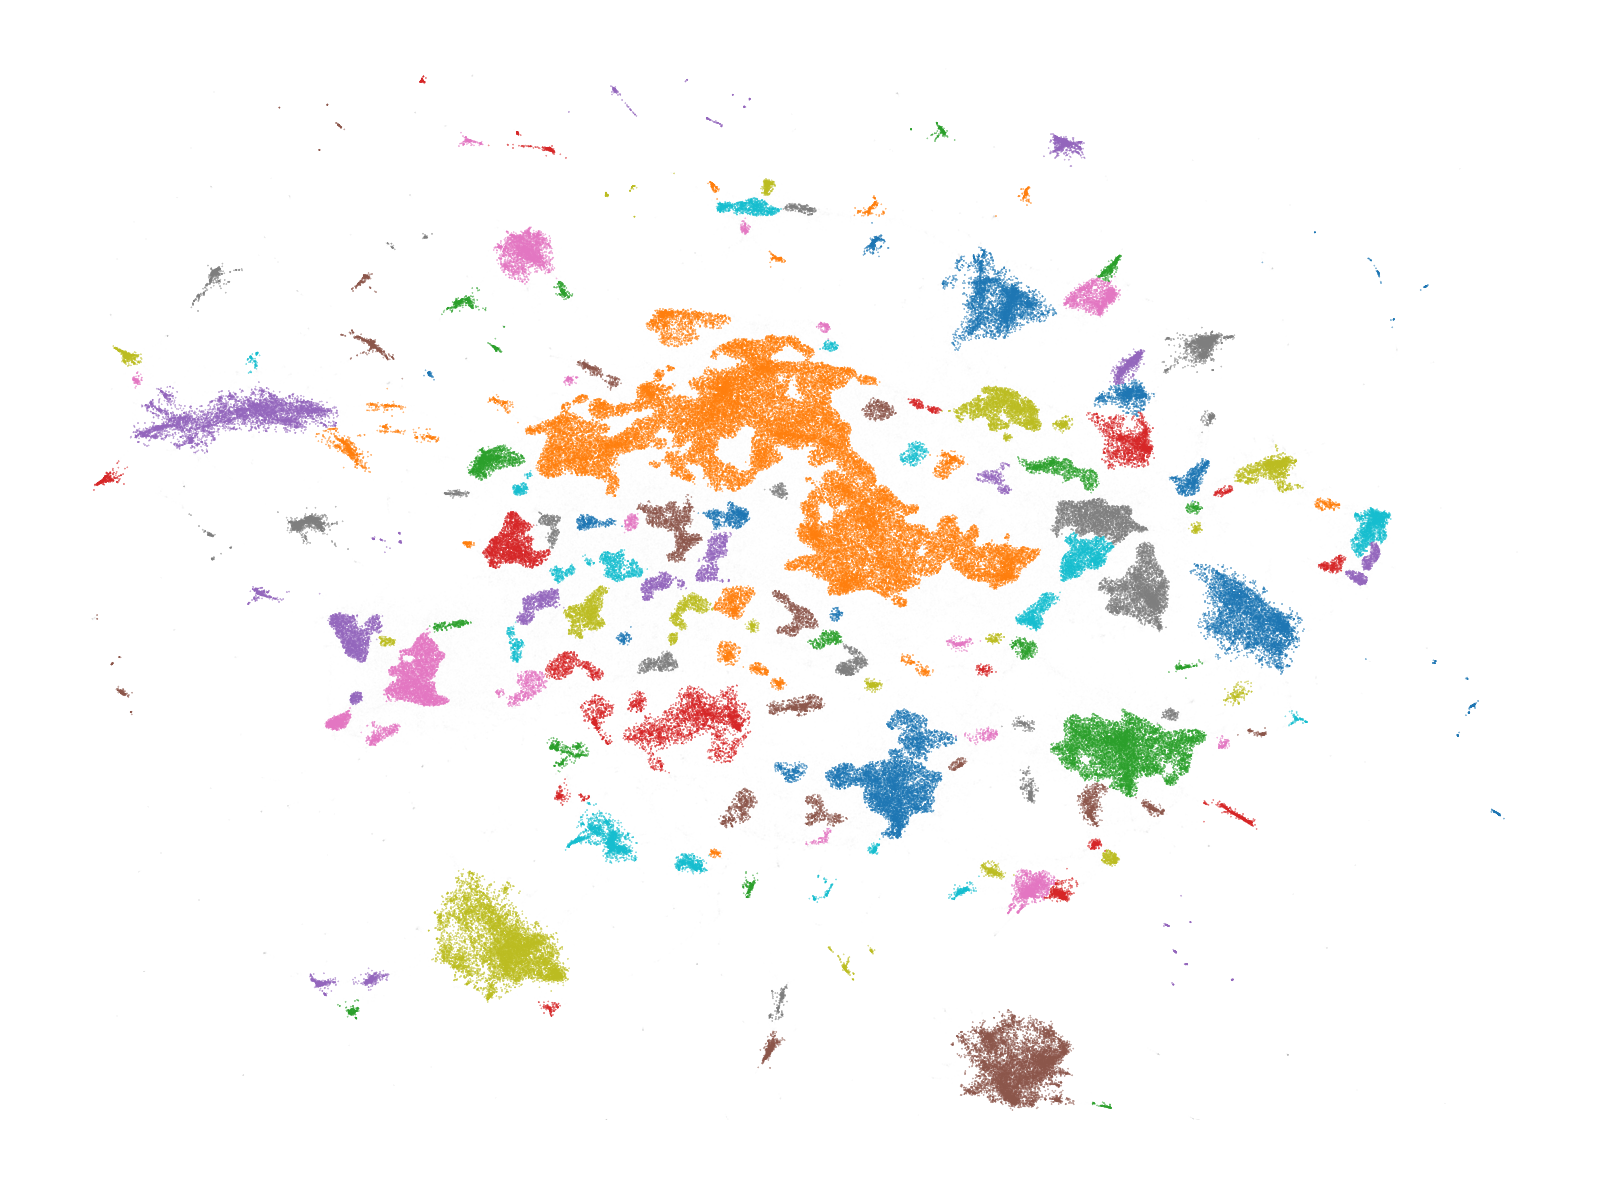
\includegraphics[width=\linewidth]{rys04/umap_5_100_100.png}
			n\_neighbors = 5
		\end{minipage}%
		\begin{minipage}{.33\textwidth}
			b)\par\medskip % chktex 10
			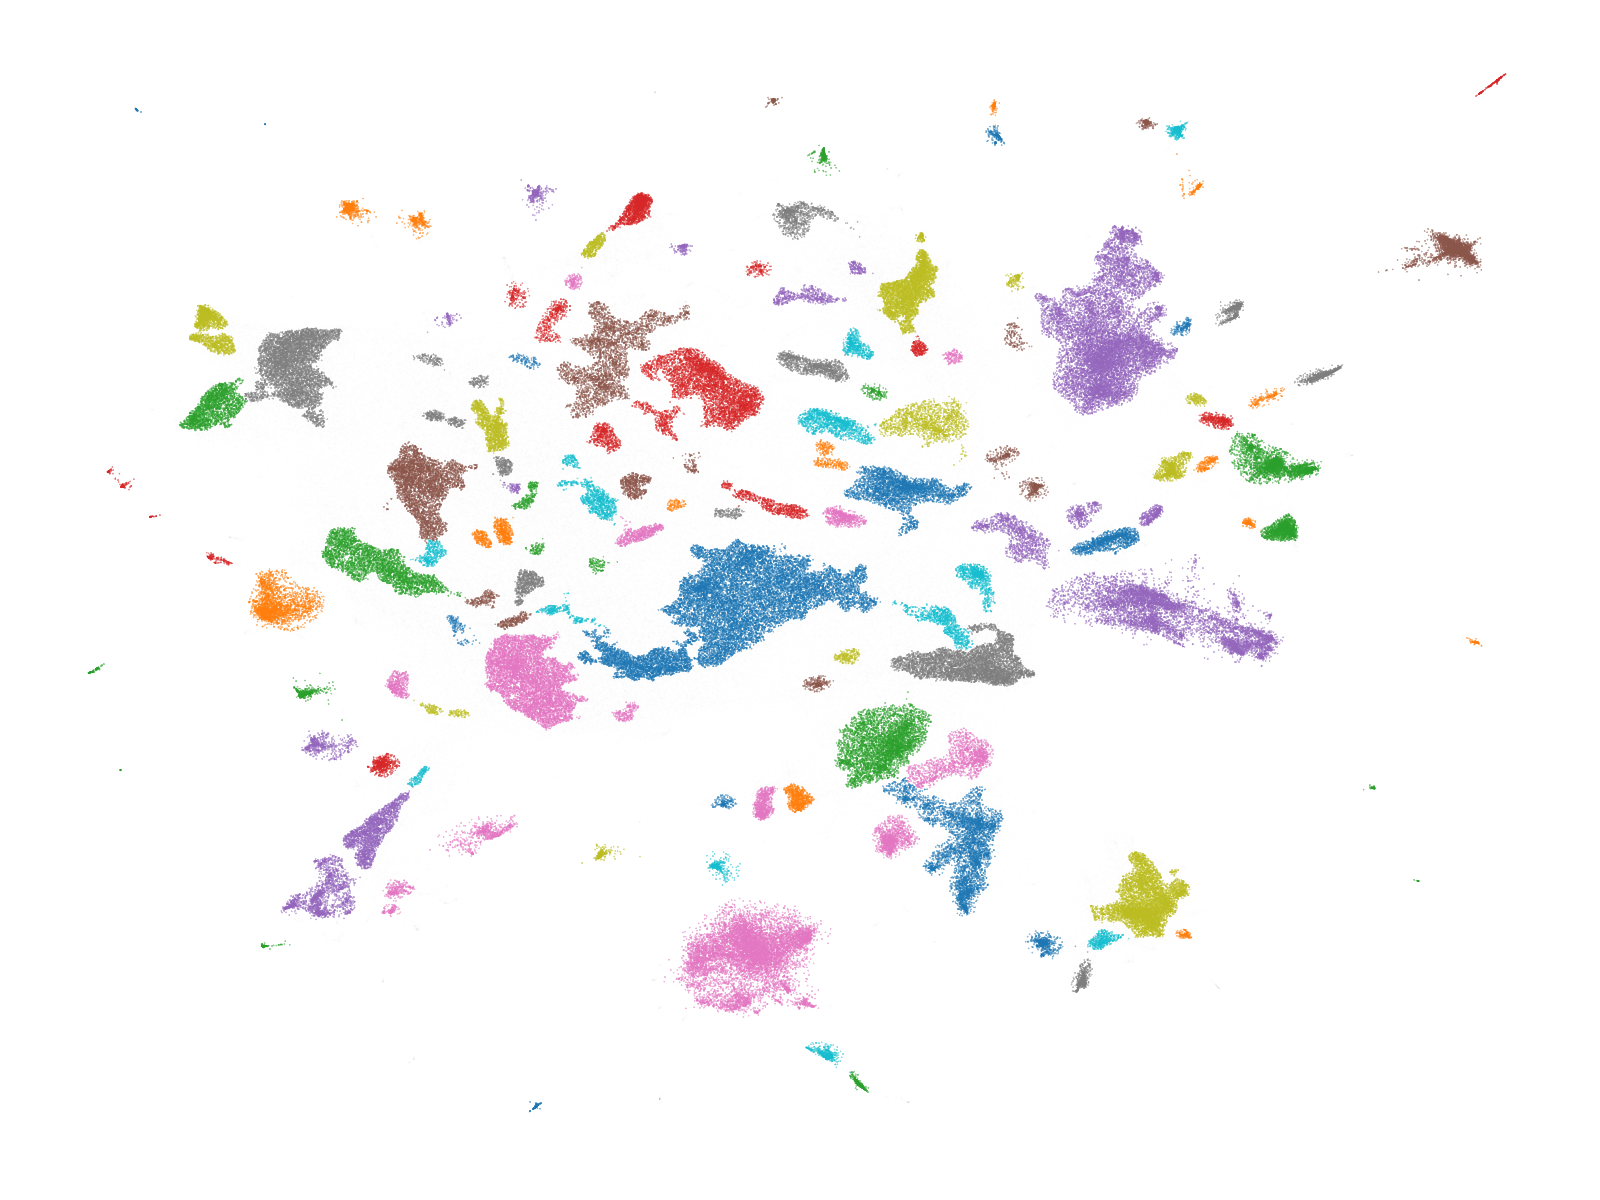
\includegraphics[width=\linewidth]{rys04/umap_15_100_100.png}
			n\_neighbors = 15
		\end{minipage}%
		\begin{minipage}{.33\textwidth}
			c)\par\medskip % chktex 10
			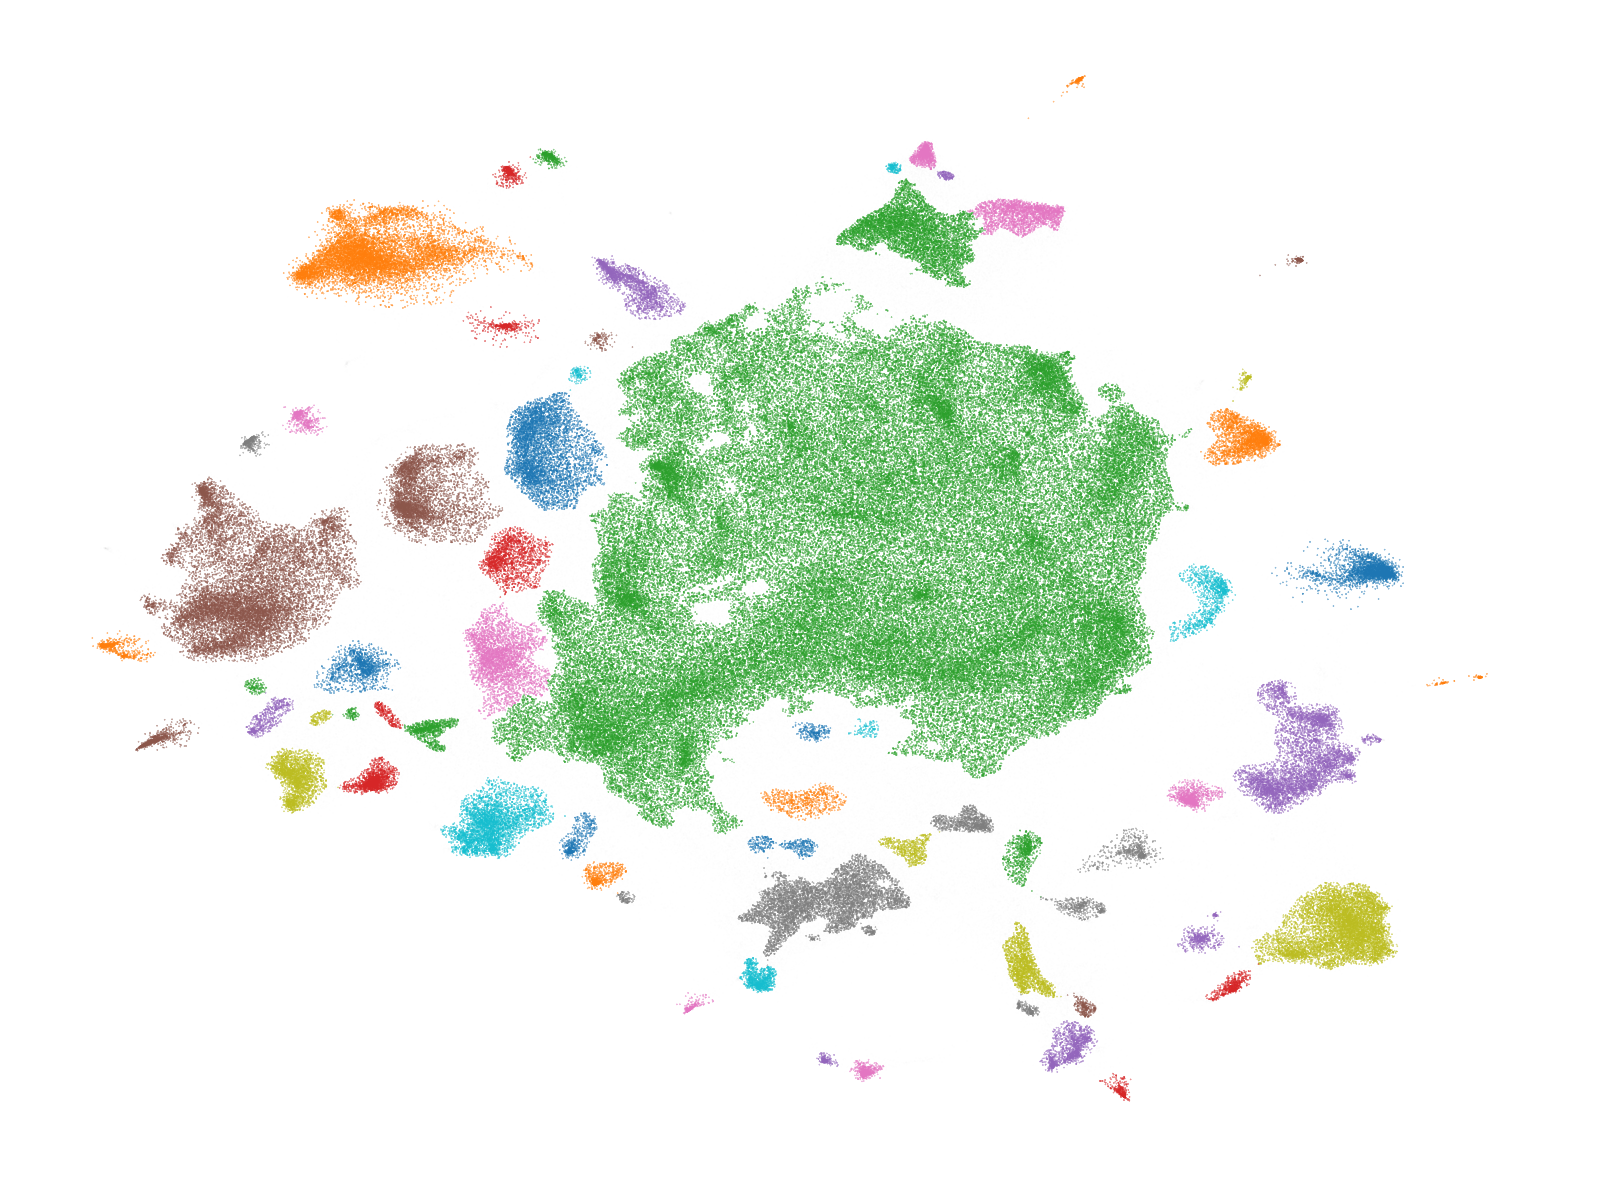
\includegraphics[width=\linewidth]{rys04/umap_100_100_100.png}
			n\_neighbors = 100
		\end{minipage}
		\caption{Dwuwymiarowa reprezentacja danych przez UMAP w zależności od wartości parametru n\_neighbors}\label{fig:umap}
	\end{figure}
	

\section{Grupowanie}
	HDBSCAN to algorytm klastrowania hierarchicznego bazujący na DBSCAN (ang.\ \emph{Density-based spatial clustering of applications with noise}).
	
	Jego działanie można opisać w pięciu krokach:
	\begin{enumerate}
		\item przekształcenie przestrzeni według gęstości punktów,
		\item osadzenie minimalnego drzewa rozpinającego graf odległości,
		\item skonstruowanie hierarchii klastrów,
		\item skondensowanie hierarchii klastrów zgodnie z minimalnym rozmiarem klastra,
		\item wydobycie stabilnych klastrów ze skondensowanego drzewa.
	\end{enumerate}
	
